\documentclass[a4paper,12pt,twoside,openright,titlepage]{book}

%Additional packages
\usepackage[utf8]{inputenc}
\usepackage[T1]{fontenc}
\usepackage[dutch,english]{babel}
\usepackage{syntonly}
\usepackage[official]{eurosym}

% Handle images
%\usepackage[graphicx]
\usepackage{graphicx}
\graphicspath{ {./images/}{./styles/} }
\usepackage{float}
\usepackage{wrapfig}

% Handle URLs
\usepackage{xurl}
\usepackage{hyperref}
\hypersetup{colorlinks=true, linkcolor=blue, citecolor=blue, filecolor=blue, urlcolor=blue, pdftitle=, pdfauthor=, pdfsubject=, pdfkeywords=}

% Tables and listings
\usepackage{multirow,tabularx}
\usepackage[table]{xcolor} % Table colors
\usepackage{scrextend}
\addtokomafont{labelinglabel}{\sffamily}
\usepackage{listings}
\usepackage{adjustbox}

% Turn on indexing
\usepackage{imakeidx}
\makeindex[intoc]

% Define colors
\usepackage{color}
\definecolor{ashgrey}{rgb}{0.7, 0.75, 0.71}



% Listing style
\lstset{
  backgroundcolor=\color{ashgrey}, % choose the background color; you must add \usepackage{color} or \usepackage{xcolor}; should come as last argument
  rulecolor=\color{black},         % if not set, the frame-color may be changed on line-breaks within not-black text (e.g. comments (green here))
  frame=single,	                   % adds a frame around the code
  basicstyle=\ttfamily,  % the size of the fonts that are used for the code
  extendedchars=true,    % lets you use non-ASCII characters; for 8-bits encodings only, does not work with UTF-8
  breakatwhitespace=true, % sets if automatic breaks should only happen at whitespace
  breaklines=true,        % sets automatic line breaking
  keepspaces=true,        % keeps spaces in text, useful for keeping indentation of code (possibly needs columns=flexible)
  columns=fullflexible,	  % Make sure no extra spaces are added.
  showstringspaces=false, % if true show spaces in strings adding particular underscores
  showspaces=false        % show spaces everywhere adding particular underscores; it overrides 'showstringspaces'
}



% Uncomment for production
% \syntaxonly

% Style
\pagestyle{headings}

% Turn on indexing
\makeindex[intoc]

% Define document
\author{D. Leeuw}
\title{Linux de grafische interface}
%\subtitle{Linux voor MBO niveau 4 en het LPI Linux Essentials examen}
%\subject{Een Praktische Gids}
\date{\today\\v.1.0.0}

\begin{document}
\selectlanguage{dutch}

\maketitle

\copyright\ 2020-2022 Dennis Leeuw\\

\begin{figure}

\includegraphics[width=0.3\textwidth]{CC-BY-SA-NC.png}
\end{figure}

\bigskip

Dit werk is uitgegeven onder de Creative Commons BY-NC-SA Licentie en laat anderen toe het werk te kopi\"eren, distribueren, vertonen, op te voeren, en om afgeleid materiaal te maken, zolang de auteurs en uitgever worden vermeld als maker van het werk, het werk niet commercieel gebruikt wordt en afgeleide werken onder identieke voorwaarden worden verspreid.


%%%%%%%%%%%%%%%%%%%
%%% Introductie %%%
%%%%%%%%%%%%%%%%%%%

\frontmatter
\chapter{Over dit Document}
Dit document behandeld Linux voor het middelbaar beroepsonderwijs in Nederland, maar kan breder ingezet worden, daar het gericht is op het behalen van het LPI Linux Essentials examen. De doelgroep is niveau 4 van het MBO, met enige kennis van computers.

\section*{Versienummering}
Het versienummer van elk document bestaat uit drie nummers gescheiden door een punt. Het eerste nummer is het major-versie nummer, het tweede nummer het minor-versienummer en de laatste is de nummering voor bug-fixes.\par
Om met de laatste te beginnen als er in het document slechts verbeteringen zijn aangebracht die te maken hebben met type-fouten, websites die niet meer beschikbaar zijn, of kleine foutjes in de opdrachten dan zal dit nummer opgehoogd worden. Als docent of student hoef je boek niet te vervangen. Het is wel handig om de wijzigingen bij te houden.\par
Als er flink is geschreven aan het document dan zal het minor-nummer opgehoogd worden, dit betekent dat er bijvoorbeeld plaatjes zijn vervangen of geplaatst/weggehaald, maar ook dat paragrafen zijn herschreven, verwijderd of toegevoegd, zonder dat de daadwerkelijk context is veranderd. Een nieuw cohort wordt aangeraden om met deze nieuwe versie te beginnen, bestaande cohorten kunnen doorwerken met het boek dat ze al hebben.\par
Als het major-nummer wijzigt dan betekent dat dat de inhoud van het boek substantieel is gewijzigd om bijvoorbeeld te voldoen aan een nieuw kwalificatiedossier voor het onderwijs of een nieuwe versie van Linux Essentials van de LPI. Een nieuw major-nummer betekent bijna altijd voor het onderwijs dat in het nieuwe schooljaar men met deze nieuwe versie aan de slag zou moeten gaan. Voorgaande versies van het document zullen nog tot het einde een schooljaar onderhouden worden, maar daarna niet meer.

\section*{Document ontwikkeling}
Het doel is door middel van open documentatie een document aan te bieden aan zowel studenten als docenten, zonder dat hier hoge kosten aan verbonden zijn en met de gedachte dat we samen meer weten dan alleen. Door samen te werken kunnen we meer bereiken.\par
Bijdragen aan dit document worden dan ook met alle liefde ontvangen. Let u er wel op dat materiaal dat u bijdraagt onder de CC BY-NC-SA licentie vrijgegeven mag worden, dus alleen origineel materiaal of materiaal dat al vrijgegeven is onder deze licentie.\par
De eerste versie is geschreven voor het ROC Horizon College.

\begin{flushleft}
\begin{table}[h!]
\centering
\begin{tabularx}{\textwidth}{ |c|c|c|X| }
\hline
	Versienummer &
	Auteurs &
	Verspreiding &
	Wijzigingen\\
\hline
	1.0.0 &
	Dennis Leeuw &
	 &
	Opdrachten naar eigen opdrachten document. Veel taal- en stijlfouten uit de teksten gehaald\\
\hline
	0.9.0 &
	Dennis Leeuw &
	 &
	Na splitsing GUI document in Intro en GUI\\
\hline
\end{tabularx}
\caption{Document wijzigingen}
\label{table:1}
\end{table}
\end{flushleft}



%%%%%%%%%%%%%%%%%
%%% De inhoud %%%
%%%%%%%%%%%%%%%%%
\tableofcontents

\mainmatter
\chapter{Inleiding}
Deze Linux cursus beoogt aan te sluiten bij het Linux Essentials examen van de LPI (Linux Professional Institute) en dient als voorbereiding op het MBO ICT Systems and Devices Expert examen. De cursus bestaat uit drie delen in het eerste deel installeren we CentOS als werkstation en leren we een grafische interface van het Linux systeem kennen. In het tweede deel werken we op de command line (CLI) en blijven we de CentOS installatie gebruiken. In deel 3 installeren we Debian en zullen we meer leren over Linux als server. De keuze om CentOS als werkstation te installeren en Debian als server is volledig willekeurig. Het doel is dat de studenten kennis maken met de rpm en dpkg package managers en leren dat het ene Linux systeem het andere niet is.

Alle Linux systemen zullen ge\"installeerd worden als virtuele machines op Virtual Box (\url{https://www.virtualbox.org/}). Door gebruik te maken van virtuele machines zijn we niet afhankelijk van de onderliggende hardware. De keuze voor VirtualBox heeft te maken met het feit dat dit product gratis te gebruiken is en beschikbaar is voor zowel Windows, Mac OS X als Linux.

Voor de CentOS machine is 15G vrije schijfruimte nodig en voor het Debian systeem 8G, wat een totaal aan 23G vrije schijfruimte vereist. Voor elke machine hebben we 2G RAM nodig, dus een totaal van 4G RAM moet vrij beschikbaar zijn.

Dit document behandelt de GUI ofwel de Graphical User Interface van Linux. Heel specifiek behandelen we de GNOME desktop omgeving zoals deze meegeleverd wordt met CentOS.


\chapter{Werken met de Desktop}
De Unix-wereld houdt erg van het paradigma ``Small is beautiful''. Daarmee bedoelen ze dat ze
graag kleine tools maken die \'e\'en ding goed doen. Dat zien we ook terug bij de grafische interface. Allereerst is er
een display server, dit is een stuk software dat ervoor zorgt dat er een grafische interface is. Het luistert naar de
muis en bestuurt de cursor en toont een grafisch scherm \ en dat is het wel zo'n beetje. Op deze grafische server
draait een window-manager. De window-manager vangt een applicatie in een frame (een window) en zorgt ervoor dat er naar
wens scrol-knoppen zijn en knopjes om het scherm te minimaliseren en/of te sluiten. Ook het achtergrondscherm is een
taak van de window-manager. Als laatste is er de desktop omgeving die zorgt voor de taakbalk, het configuratiescherm en
alle andere zaken die nodig zijn om van een desktop te kunnen spreken.

{\selectlanguage{dutch}
Als we dit allemaal hebben hebben we een desktop omgeving waarbinnen applicaties kunnen draaien.}

{\selectlanguage{dutch}
Er zijn twee dominante desktop omgevingen beschikbaar op de verschillende Linux distributies en dat zijn KDE en GNOME.
Naast deze twee zijn er nog vele verschillende anderen, maar die zullen we hier niet bespreken.}

{\selectlanguage{dutch}
\foreignlanguage{dutch}{KDE was de eerste van de twee genoemde desktopomgevingen en is gebaseerd op de Qt-library. In
het begin was de Qt-library geen open source vandaar dat er een concurrerent project is ontstaan. Later is het met Qt
helemaal goed gekomen en nu behoort ze tot de open source gemeenschap.}}

{\selectlanguage{dutch}
GNOME was het concurrerende project dat gestart werd omdat Qt niet open source was. Voor GNOME tot stand kwam was er een
open source fotomanipulatiepakket dat The \index{GIMP}GIMP heet, zie later in dit hoofdstuk. Om het pakket te kunnen
maken hadden de ontwikkelaars een grafische library ontwikkeld die GTK werd genoemd. Veel van wat er nodig is voor een
desktop zat daar al in en dus gebruikte het GNOME project de GTK-library als basis.}

{\selectlanguage{dutch}
\foreignlanguage{dutch}{De grafische interface kan enorm verschillen per distributie. Het maakt al enorm veel verschil
of je KDE of GNOME gebruikt als desktop omgeving. Laat je hierdoor niet imponeren, het wijst zich vaak vanzelf. KDE
ligt qua interface het dichtst tegen Windows aan, en zal dus het makkelijkst zijn om naar over te stappen. CentOS
gebruikt GNOME en vergt iets meer doorzettingsvermogen om te doorgronden.}}

{\selectlanguage{dutch}
\foreignlanguage{dutch}{Mocht het scherm in zijn screensaver vallen dan kan je door te clicken een scherm krijgen waarop
de tijd te zien is en met de {\textless}Enter{\textgreater} toets kom je op een login scherm en kan je in loggen met je
gebruikers wachtwoord.}}

{\selectlanguage{dutch}
\foreignlanguage{dutch}{Door op Activities te clicken krijg je extra scherm elementen te zien. Het nog een keer
aanclicken van Activities verbergt de elementen weer waardoor je meer ruimte op je scherm hebt voor applicaties.}}



\begin{figure}[H]
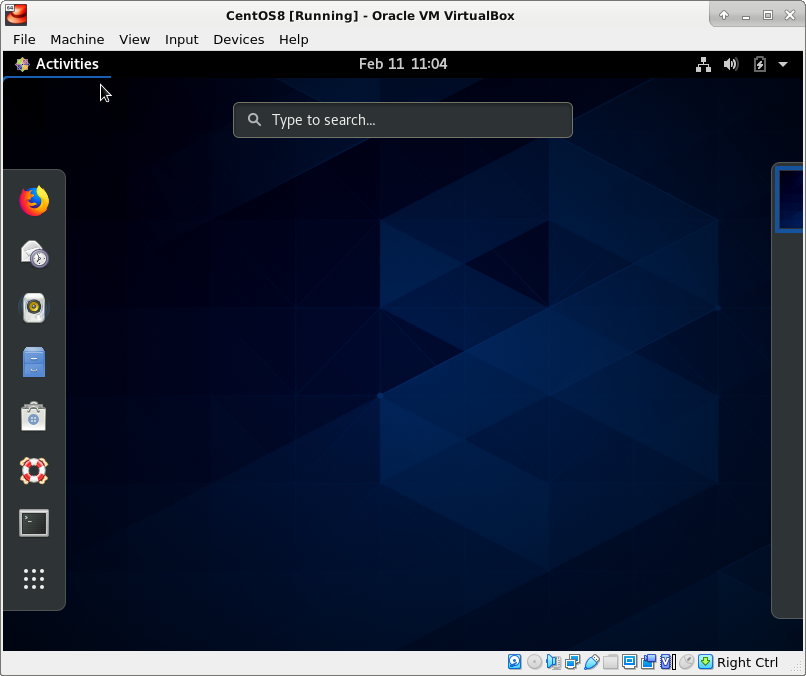
\includegraphics[width=0.9\textwidth]{linuxreader-img013.png}
\end{figure}
\begin{figure}[H]
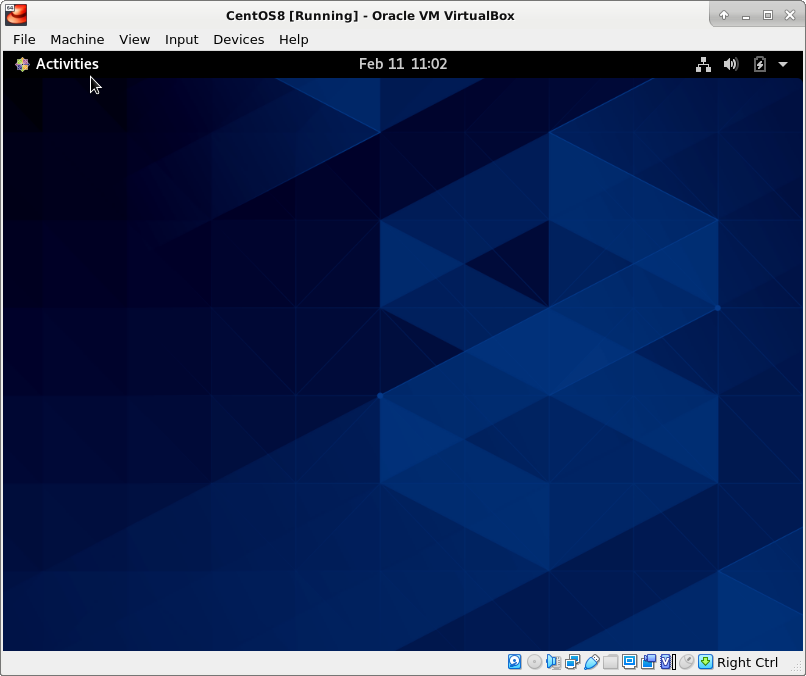
\includegraphics[width=0.9\textwidth]{linuxreader-img014.png}
\end{figure}

\section{Zoeken van bestanden of applicaties}
Met alle elementen op het scherm kan je de searchbar gebruiken om te zoeken op applicaties en bestanden. Als je zoekt op
Word, een Microsoft applicatie die niet op Linux beschikbaar is, dan vind je LibreOffice Writer een gratis en open
source alternatief. Start de applicatie op.

{\selectlanguage{dutch}
Neem de tekst over van het plaatje hierboven en zorg dat dit een eerste hoofdstuk titel wordt door de stijl te
veranderen. We gaan het document later vullen. Selecteer File en Save as{\dots} om het bestand op te slaan als
Document1.}

\begin{figure}[H]
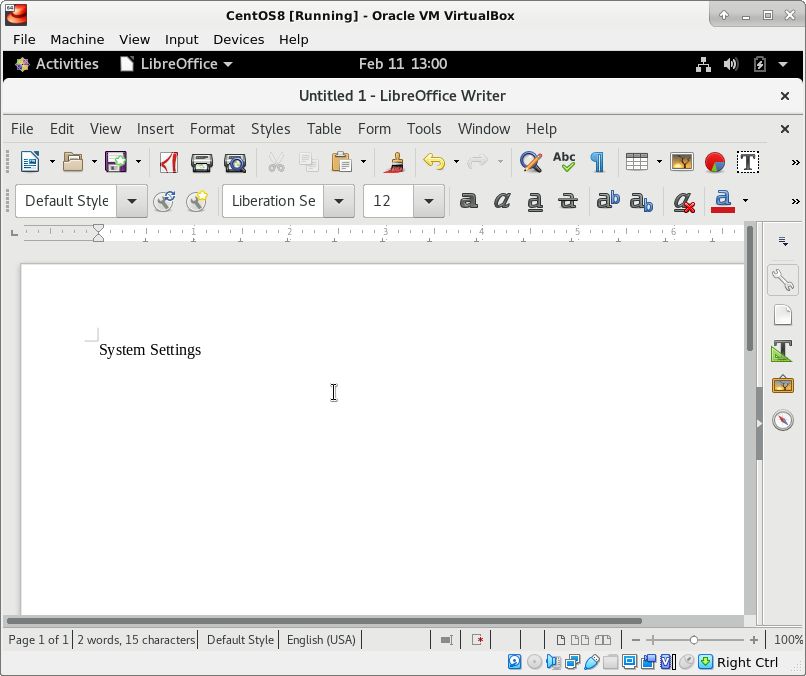
\includegraphics[width=0.9\textwidth]{linuxreader-img015.png}
\end{figure}
{\selectlanguage{dutch}
\foreignlanguage{dutch}{Meer over LibreOffice en de verschillende onderdelen van dit office pakket komt later aan de
orde als we Office Pakketten gaan bespreken. Nu concentreren we ons eerst op de beschikbare scherm elementen.}}

\section{Systeem configuratie}
Op de donkere balk waarop ook Activities staat vind je aan de rechterkant een naar beneden wijzend driehoekje. Het
aanklikken van het driehoekje geeft een menu met daarop een overzicht van de helderheid van het scherm, aan welk
netwerk je gekoppeld bent, als je een laptop gebruikt wat de batterij status is, je loginnaam en drie knopjes die je
van links naar rechts toegang geven tot de systeemsettings, het locken van je scherm en het uitzetten of herstarten van
je machine.



\begin{figure}[H]
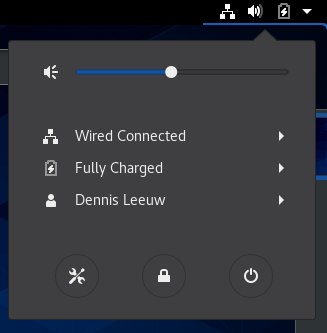
\includegraphics[width=0.9\textwidth]{linuxreader-img016.png}
\end{figure}
{\selectlanguage{dutch}
Selecteer Settings, scroll naar beneden naar Devices en selecteer deze, click dan op Displays. Trek het scherm los van
de topbar en schuif hem naar links. Click op de 800x600 resolutie en zet deze naar 1024x768}

{\selectlanguage{dutch}
\foreignlanguage{dutch}{Click op de Apply knop rechtsboven aan het scherm en daarna op Keep Settings. Natuurlijk mag je
resolutie ook hoger zetten, maar de minimale resolutie waarmee GNOME op CentOS 8 op een virtual machine prettig werkt
zonder dat je steeds met windows moet slepen is 1024x768. Selecteer {\textless} in de balk van Devices om terug te
komen in het hoofdmenu voor Settings. Loop door de verschillende opties om te ervaren waar je welke configuratie items
kan vinden en wijzigen.}}

\begin{figure}[H]
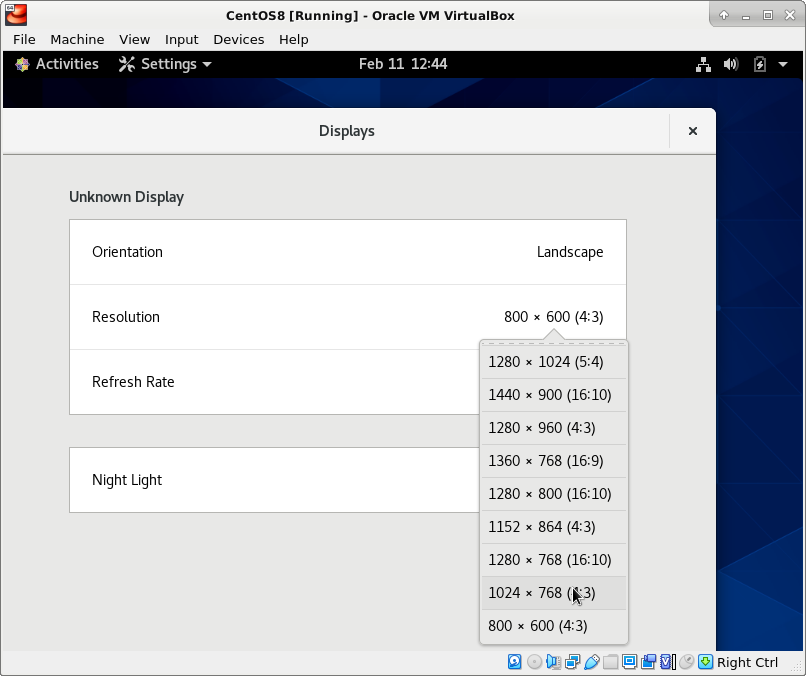
\includegraphics[width=0.9\textwidth]{linuxreader-img017.png}
\end{figure}
{\selectlanguage{dutch}
\foreignlanguage{dutch}{[TODO] Opdracht met documentatie in Writer om iets op te zoeken en te documenteren in Document1.
}}


\section{The Dash}
Aan de linkerkant van je scherm heb je de Dash, ook bekend als de Dock, applicatie bar of taskbar. Als je met je muis over de iconen van de taskbar gaat dan zie je per icoon wat deze betekent. Van boven naar beneden kom je het volgende tegen.

\begin{figure}[H]

\includegraphics[width=0.7811in,height=4.7398in]{linuxreader-img018.png}
\end{figure}
\begin{itemize}
\item Firefox -- een webbrowser
\item Evolution -- Een e-mail client
\item Rhythmbox -- een muziekspeler
\item Files -- Bestandsbrowser
\item Software -- Softwarebeheer
\item Help -- Documentatie
\item Terminal -- Toegang tot de console
\item Show applications -- een beperkt overzicht van beschikbare applicaties.
\end{itemize}

In de volgende hoofdstukken zullen we deze elementen doorlopen maar in een bredere context. We zullen bijvoorbeeld niet alleen Firefox behandelen, maar webbrowsers in zijn algemeenheid.


\section{Bestandsbrowser}
De filebrowser\index{Filebrowser}\index{Desktop!Filebrowser} kan gevonden worden op de Dash met het archief icon.
\begin{figure}[H]
	\centering
\includegraphics{filebrowser-dash.png}
	\caption{Filebrowser Icoon}
	\label{fig:de_filebrowser_icon}
\end{figure}

De filebrowser geeft je de mogelijkheid om op een grafische manier door de mappen en bestanden van het systeem te bladeren.
\begin{center}
\begin{figure}[H]
\includegraphics[width=\linewidth]{filebrowser.png}
	\caption{Filebrowser}
	\label{fig:de_filebrowser}
\end{figure}
\end{center}




\chapter{Installeren en updaten van software}
Via het software icon op de dash kan je de applicatie opstarten om de software op je systeem te beheren.
\begin{figure}[H]
\includegraphics{software-dash.png}
\end{figure}
Je kan er applicaties mee toevoegen aan je systeem of juist van je systeem verwijderen.


\section{Installeren van GIMP}
\begin{figure}[H]
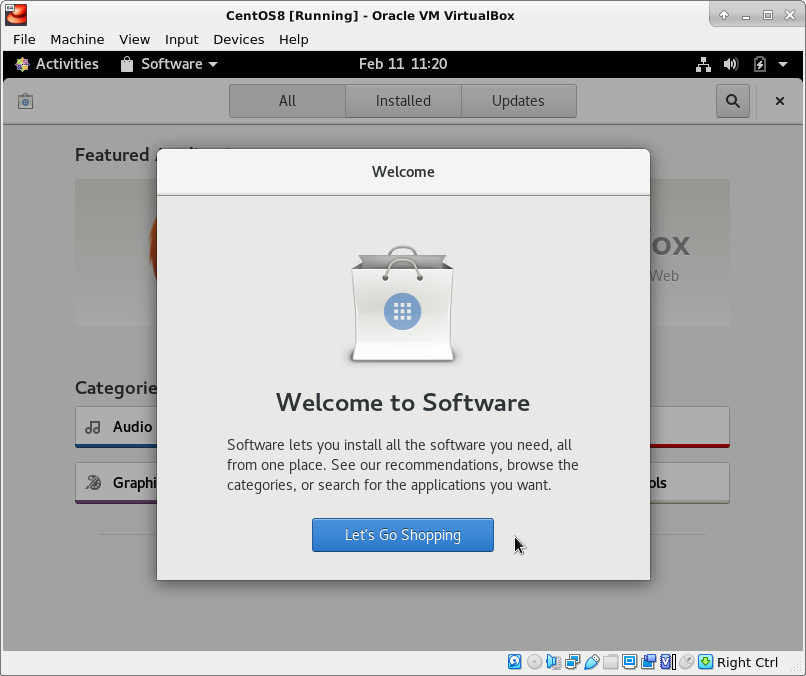
\includegraphics[width=0.9\textwidth]{linuxreader-img019.png}
\end{figure}
{\selectlanguage{dutch}
Rechtsboven kunnen we zoeken op een applicatie, we kunnen echter ook kiezen voor applicaties uit een Categorie. Klikken
we op Graphics \& Photography. Dan vinden we tussen de opties de Gimp. Selecteer de Gimp en klik Install. Er zal
gevraagd worden om het root-wachtwoord, na dit ingevoerd te hebben begint de installatie.}

{\selectlanguage{dutch}
Hierna kan je Software afsluiten of direct de Gimp opstarten.}

\begin{figure}
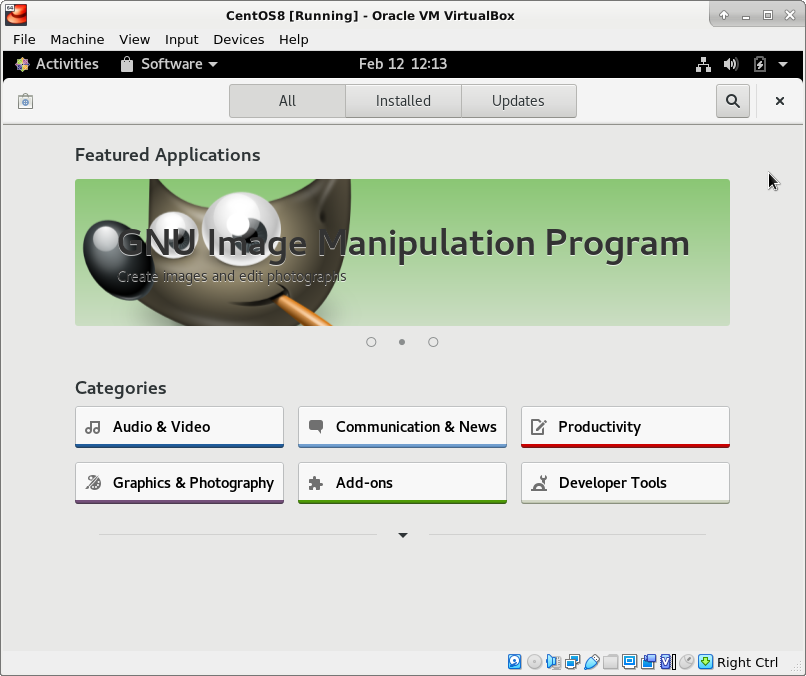
\includegraphics[width=0.9\textwidth]{linuxreader-img020.png}
\end{figure}

\section{Show applications}
Dit geeft een beperkt overzicht van de beschikbare applicaties. Voor snelle toegang tot de meest gebruikte applicaties
is dit een prima oplossing, verder is het makkelijker om gebruik te maken van de zoekfunctie zoals deze eerder in dit
document beschreven is.



\chapter{Internet}
\section{Webbrowsers}
Een populaire browser is Mozilla \index{Firefox}Firefox. Het KDE-project heeft zijn eigen webbrowser. De KDE browser bestaat uit een engine
en en een interface. De engine is een library die alle benodigde functies voor het afhandelen van webpagina's heeft.
Het is ooit begonnen als KHTML. \ , de engine van deze browser,
\index{WebKit}WebKit wordt inmiddels ook door Apple gebruikt voor
zijn Safari browser.

Toen Google zijn eigen webbrowser ontwikkelde werd de basis hiervan vrij gegeven als open source
browser met de naam \index{Chromium}Chromium. Google gebruikt zelf
ook deze basis voor zijn Chrome browser, maar voegt daar nog wat eigen elementen aan toe. De open source versie is ook
op Linux te gebruiken en wordt door veel distributies meegeleverd en is makkelijk later te installeren.

[TODO] Basisgebruik firefox


\section{E-mail clients}
Mozilla levert naast de browser Firefox ook een open source \index{e-mail!e-mail client}e-mail client met de naam
\index{Thunderbird}Thunderbird dit is een volwaardige e-mail client inclusief kalenderfunctionaliteit.

Een e-mail client die erg lijkt op Microsoft Outlook is \index{Evolution}Evolution. Sinds versie 2.8 is het onderdeel
van het GNOME project en Evolution is dan ook standaard ge\"installeerd op CentOS.

Evolution en Thunderbird draaien ook op Windows en Mac OS X.

Het KDE project heeft daarnaast ook zijn eigen e-mail client en die heet \index{KMail}KMail.

Standaard zijn er dus voor Linux al vele e-mail clients om uit te kiezen. Als je Op Internet gaat zoeken zijn er nog veel meer smaken beschikbaar. Dat is een van de
vele voordelen van open source, anderen zeggen een nadeel, er zijn enorm veel keuzes.


\chapter{Office Applicaties}
\section{Office pakketten}\index{Office pakketten}
Jaren lang was het meest gebruikte en dominante office pakket dat van Microsoft. Het was
beschikbaar voor Windows en Mac OS, maar niet voor Linux systemen. Oorspronkelijk had een Duitse student, Marco
B\"orries, StarWriter ontwikkeld om zijn studie in te documenteren. Later richtte hij een bedrijf op genaamd Star
Division en werd het een office pakket met de naam StarOffice. Het bedrijf werd in 1999 opgekocht door Sun Microsystems
die het pakket open source maakte onder de naam OpenOffice.org.

{\selectlanguage{dutch}
\foreignlanguage{dutch}{In 2009 werd Sun Microsystems gekocht door Oracle. Er was veel twijfel over wat Oracle met
OpenOffice.org wilde en dat zorgde voor een fork, een kopie van de code, die bekend werd onder de naam LibreOffice in
2010 en beheerd wordt door The Document Foundation. Oracle bracht }\foreignlanguage{dutch}{uiteindelijk in 2011 de code
van OpenOffice.org onder bij de Apache Foundation, helaas zat toen het merendeel van de ontwikkelaars al bij
LibreOffice. Beide projecten bestaan nog steeds, maar de meeste distributies leveren LibreOffice mee.}}

{\selectlanguage{dutch}
\foreignlanguage{dutch}{LibreOffice gebruikt standaard het Open Document Format voor al zijn documenten en is gratis
beschikbaar. Voor Linux, Mac OS X en Windows kan je het pakket vanaf de website downloaden
}\href{https://www.libreoffice.org/}{https://www.libreoffice.org}\foreignlanguage{dutch}{, maar dat hoeven wij niet te
doen omdat we het al meege\"installeerd hebben tijdens de installatie van CentOS.}}

{\selectlanguage{dutch}
LibreOffice bevat de volgende software onderdelen}

\begin{itemize}
\item {\selectlanguage{dutch}
Writer -- Tekstverwerking}
\item {\selectlanguage{dutch}
Calc -- Spreadsheets}
\item {\selectlanguage{dutch}
Impress -- Presentaties}
\item {\selectlanguage{dutch}
Draw -- Tekenpakket}
\item {\selectlanguage{dutch}
Math -- Een formule editor}
\item {\selectlanguage{dutch}
Base -- Database}
\end{itemize}
{\selectlanguage{dutch}
LibreOffice maakt standaard gebruik van het Open Document Format. Een officieel erkent en gestandaardiseerd
bestandsformaat dat er voor zorgt dat data altijd weer te lezen is omdat exact beschreven is hoe een document opgebouwd
moet zijn. De belangrijkste bestandsformaten zijn:}

\begin{itemize}
\item {\selectlanguage{dutch}
odt -- Open Document Text}
\item {\selectlanguage{dutch}
ods -- Open Document Spreadsheet}
\item {\selectlanguage{dutch}
odp -- Open Document Presentation}
\item {\selectlanguage{dutch}
odi -- Open Document Image, bitmap format}
\item {\selectlanguage{dutch}
odg -- Open Document Graphic, vector format}
\item {\selectlanguage{dutch}
odf -- Open Document Formula}
\item {\selectlanguage{dutch}
odb -- Open Document Database}
\end{itemize}

\section{Grafische applicaties}


\subsection{The GIMP}\index{GIMP}\index{The GIMP}
\begin{figure}[H]
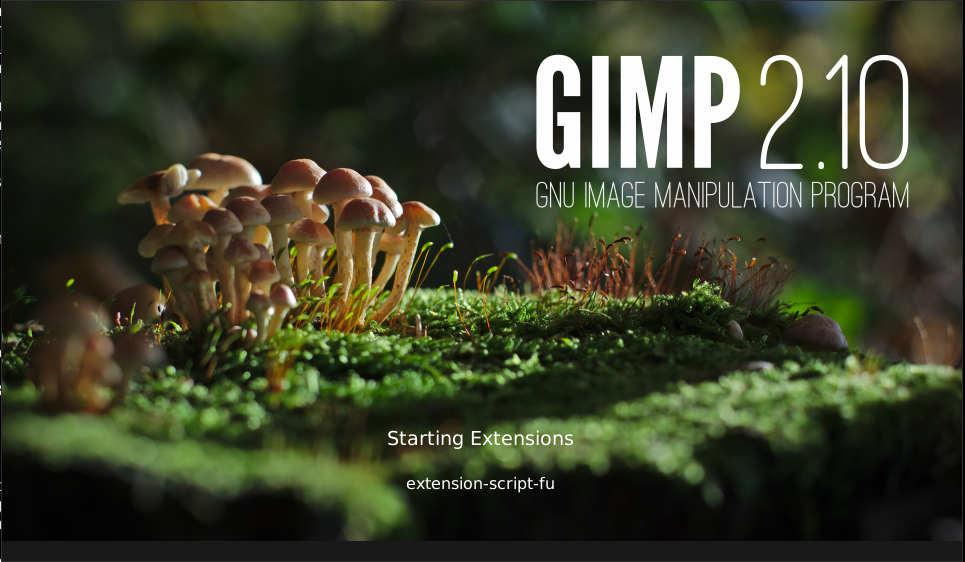
\includegraphics[width=\linewidth]{Gimp-splash.png}
\end{figure}

De GIMP is een applicatie om foto's te bewerken. Je kan het vergelijken met Photoshop van Adobe. Voor diegene die gewend zijn om te werken met Photoshop zal de interface aan de ene kant bekend voorkomen en aan de andere kant net even anders zijn.

\begin{figure}[H]
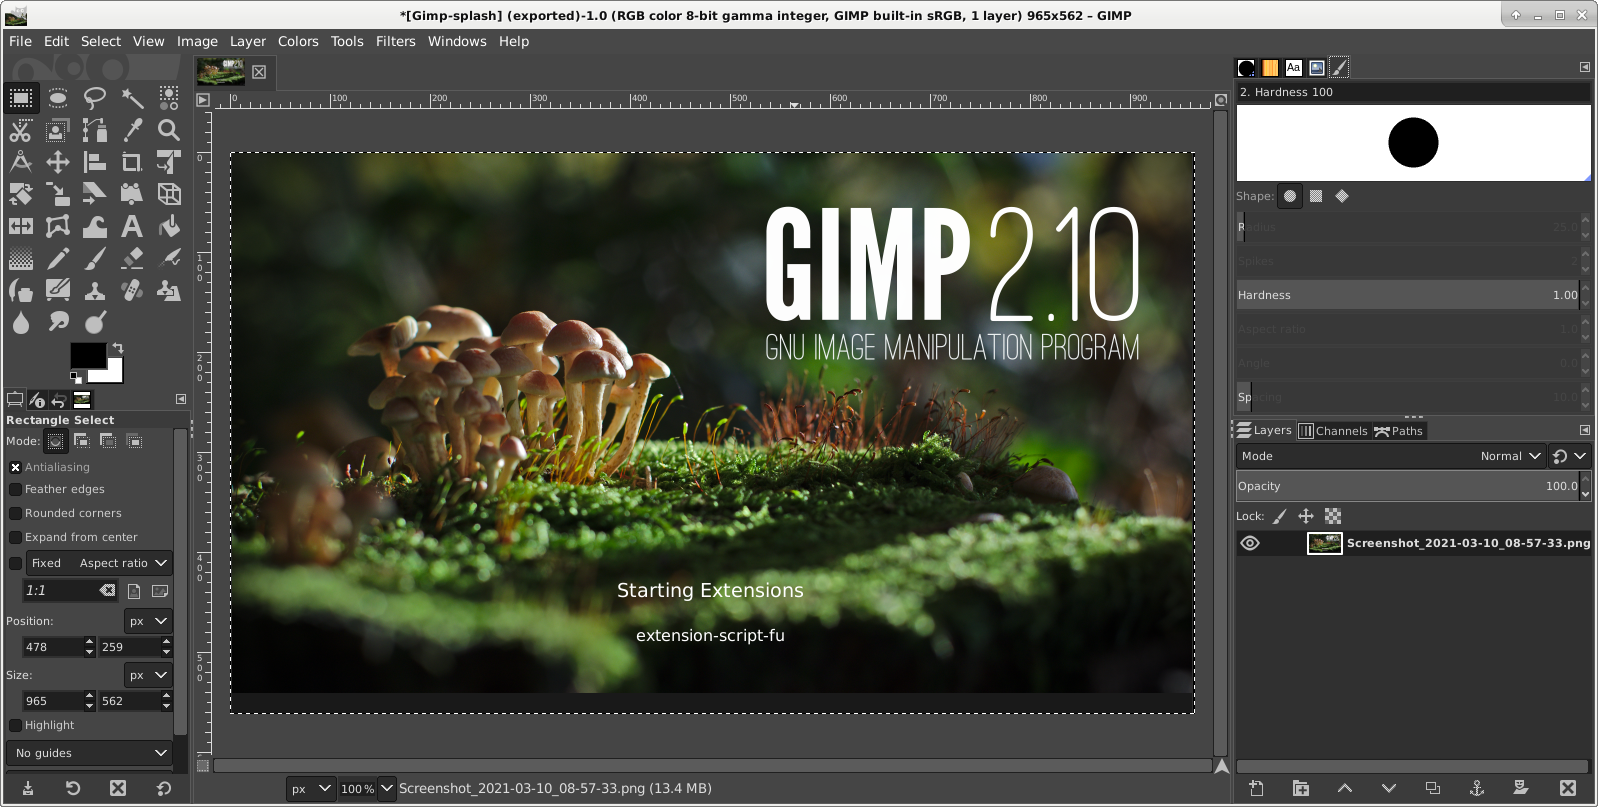
\includegraphics[width=\linewidth]{Gimp-work.png}
\end{figure}

\subsection{Inkscape}\index{Inkscape}
\index{Inkscape}Inkscape is een applicatie om tekeningen in vectoren te maken. Het bouwt een tekening dus niet op in pixels zoals bijvoorbeeld BMP, jpeg of PNG, maar doet dit door punten met vectoren te beschrijven, hierdoor zijn tekeningen ``oneindig'' schaalbaar zonder kwaliteitsverlies.
\begin{figure}[H]
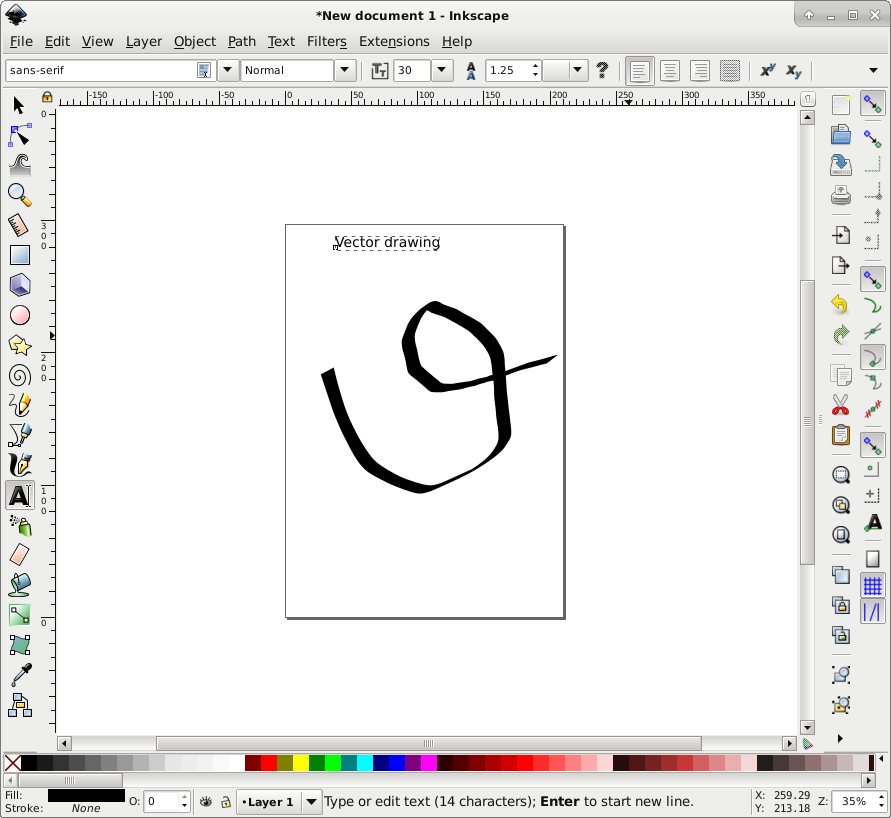
\includegraphics[width=\linewidth]{Inkscape-work.png}
\end{figure}



\section{Scribus}\index{Scribus}
Een open source document opmaak pakket is \index{Scribus}Scribus. Het is vergelijkbaar met Adobe Pagemaker.



\chapter{Multimedia}
Het Linux systeem is rijk aan multimedia applicaties. Omdat van ouds veel codecs, vertallers van analoog naar digitaal, voorzien waren van patenten zijn er ook veel open source en patent vrije codecs ontwikkeld. Voor audio zijn dat o.a. FLAC (Free and Lossless Audio Codec) en Ogg Vorbis dat een vervanger is voor bijvoorbeeld MP3. Voor video is er Theora ontwikkeld. Al deze standaarden zijn ondergebracht bij de Xiph Foundation, een non-profit organisatie die zich bezig houd met de ontwikkeling en het ondersteunen van het ontwikkelen van open standaarden op het gebied van multimedia.

\section{Muziekspelers}\index{muziekspelers}
Rhythymbox\index{rhythmbox} is een muziekspelen ontwikkeld voor de GNOME-desktop. Het is ge\"inspireerd op de iTunes applicatie en lijkt er dan ook erg op. Een andere bekende muziekspeler is Quod Libet\index{Quod Libet} dat geschreven is in python en daardoor draait op Windows, Mac OS X en Linux.

\begin{center}
\begin{figure}[H]
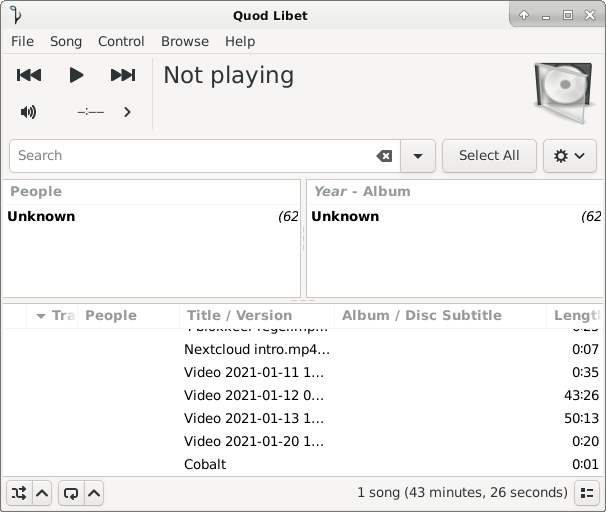
\includegraphics[]{quod_libet-working.png}
\caption{Quod Libet}
\end{figure}
\end{center}


\section{VLC}\index{VLC}\index{Video LAN Client}
VLC is uitgegroeid tot een cross-platform multimedia speler die veel gebruikt wordt om films mee te kijken. VLC draait op Linux, Mac OS X en Windows. VLC kan films ook spelen vanaf CD, DVD en BluRay. Het ondersteunt vele codecs en bestandsformaten. VLC kan je ook als server gebruiken om films te streamen over het netwerk.

\begin{center}
\begin{figure}[H]
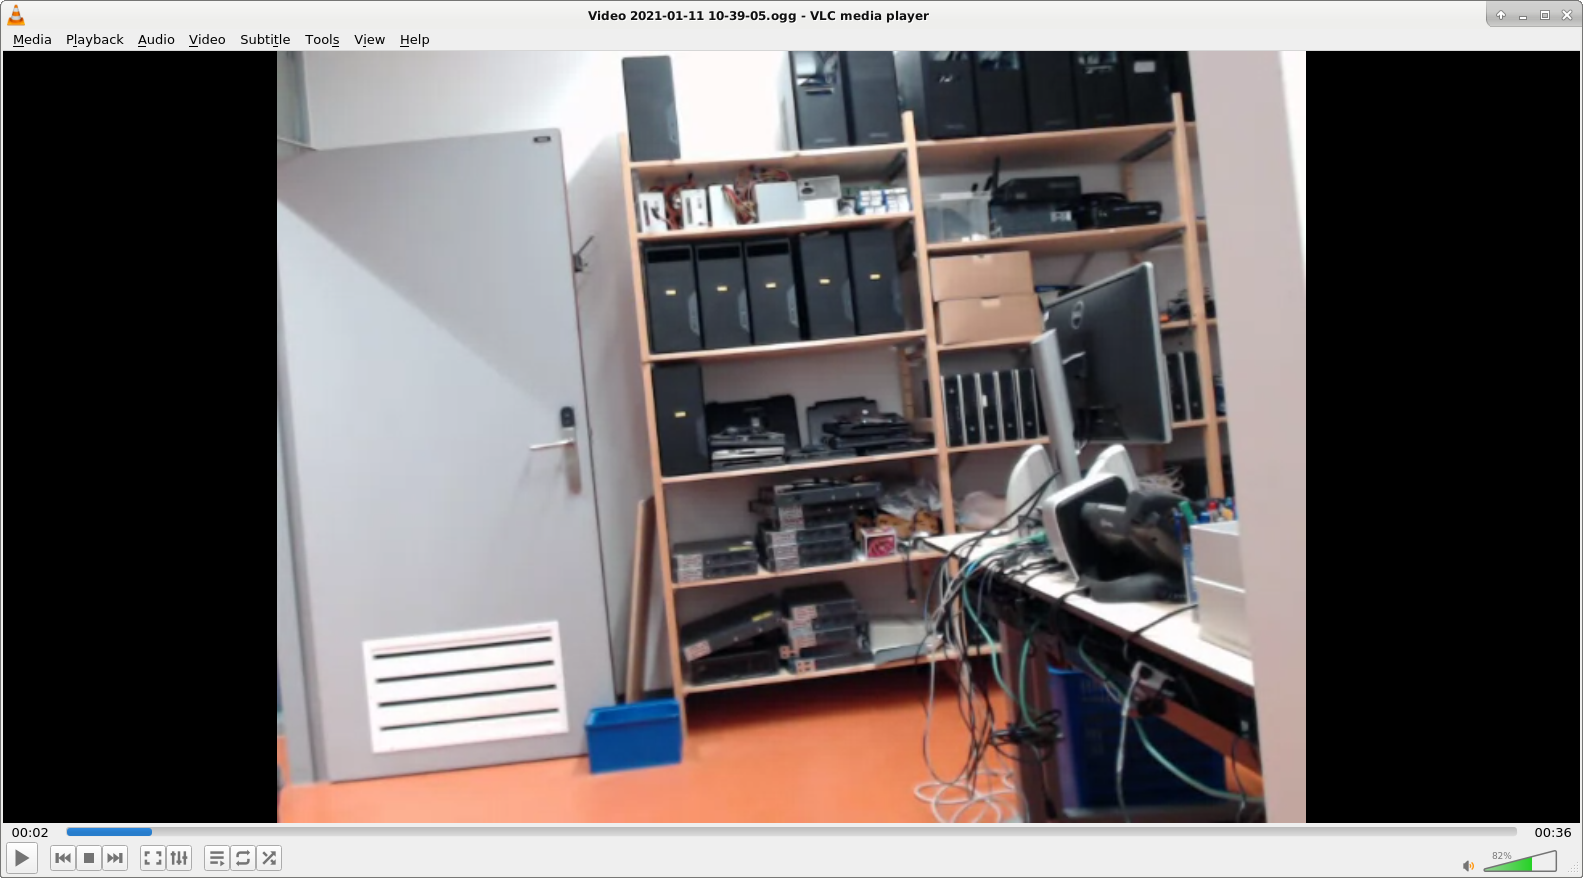
\includegraphics[width=0.9\textwidth]{VLC-working.png}
\caption{VLC}
\end{figure}
\end{center}

\section{KODI}\index{KODI}
Kodi is een multimedia-player. Oorspronkelijk is het ontwikkeld voor de Xbox en heette toen ook XBMC (XBox Media Center). Later werd XBMC door ontwikkeld voor Windows, Mac OS X en Linux en na versie 13 vernaderde de naam in Kodi. Met Kodi kan je televisie kijken via Internet (of de kabel als een televisie-kaart in je computer hebt), je kan het gebruiken als videorecorder en natuurlijk om je eigen films en muziek bestanden af te spelen.



\chapter{Naar de command line}
\section{Terminal}
De terminal applicatie wordt gebruikt om op de command line terecht te komen. Deze applicatie komt in het CLI document uitgebreid aan
de orde.

\begin{figure}
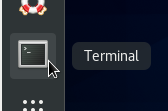
\includegraphics{linuxreader-img021}
\caption{Terminal op de Dash}
\end{figure}


%%%%%%%%%%%%%%%%%%%%%
%%% Index and End %%%
%%%%%%%%%%%%%%%%%%%%%
\backmatter
\printindex
\end{document}

%%% Last line %%%
